% File tacl2018v2.tex
% Sep 20, 2018

% The English content of this file was modified from various *ACL instructions
% by Lillian Lee and Kristina Toutanova
%
% LaTeXery is mostly all adapted from acl2018.sty.

\documentclass[11pt,a4paper]{article}
\usepackage{times,latexsym}
\usepackage{url}
\usepackage[T1]{fontenc}

%% Package options:
%% Short version: "hyperref" and "submission" are the defaults.
%% More verbose version:
%% Most compact command to produce a submission version with hyperref enabled
%%    \usepackage[]{tacl2018v2}
%% Most compact command to produce a "camera-ready" version
%%    \usepackage[acceptedWithA]{tacl2018v2}
%% Most compact command to produce a double-spaced copy-editor's version
%%    \usepackage[acceptedWithA,copyedit]{tacl2018v2}
%
%% If you need to disable hyperref in any of the above settings (see Section
%% "LaTeX files") in the TACL instructions), add ",nohyperref" in the square
%% brackets. (The comma is a delimiter in case there are multiple options specified.)

\usepackage[]{acl2021}

%%%% Material in this block is specific to generating TACL instructions
\usepackage{xspace,mfirstuc,tabulary}
\newcommand{\dateOfLastUpdate}{Sept. 20, 2018}
\newcommand{\styleFileVersion}{acl2021}

\newcommand{\ex}[1]{{\sf #1}}

\newif\iftaclinstructions
\taclinstructionsfalse % AUTHORS: do NOT set this to true
\iftaclinstructions
\renewcommand{\confidential}{}
\renewcommand{\anonsubtext}{(No author info supplied here, for consistency with
TACL-submission anonymization requirements)}
\newcommand{\instr}
\fi


% Standard package includes
\usepackage{times}
\usepackage{latexsym}

% For proper rendering and hyphenation of words containing Latin characters (including in bib files)
\usepackage[T1]{fontenc}
% For Vietnamese characters
% \usepackage[T5]{fontenc}
% See https://www.latex-project.org/help/documentation/encguide.pdf for other character sets

% This assumes your files are encoded as UTF8
\usepackage[utf8]{inputenc}

% This is not strictly necessary, and may be commented out,
% but it will improve the layout of the manuscript,
% and will typically save some space.
\usepackage{microtype}

\usepackage{tabularx}
\usepackage{booktabs}
\usepackage{amsmath}
\usepackage{amssymb}
\usepackage{multirow}
\usepackage{listings}
\usepackage{newfloat}
\usepackage[framemethod=TikZ]{mdframed}
\usepackage{hyperref}
\usepackage{microtype}  % OD added: better typography, uses 
\usepackage{caption}
\usepackage{arydshln}

\usepackage{pifont}
\newcommand{\cmark}{\ding{51}}%
\newcommand{\xmark}{\ding{55}}%

\DeclareFloatingEnvironment[placement={!ht},name=Example]{example}
\captionsetup[example]{aboveskip=2pt}%,labelfont=bf}
\newcommand{\exampleref}[1]{Example~\ref{#1}}
\newcommand{\multiwoz}[0]{MultiWOZ 2.0\xspace}
\newcommand{\multiwozn}[0]{MultiWOZ 2.1\xspace}
\newcommand{\taskmaster}[0]{Taskmaster-1\xspace}
\newcommand{\schema}[0]{Schema-Guided Dialogue\xspace}
% XXX we can replace this with AuGPT later
\newcommand{\augpt}[0]{our model\xspace}
\newcommand{\Augpt}[0]{Our model\xspace}
\newcommand{\code}[1]{\texttt{#1}}

\mdfdefinestyle{ExampleFrame}{%
    nobreak=true,
    innertopmargin=4pt,
    innerbottommargin=4pt,
    innerrightmargin=4pt,
    innerleftmargin=4pt,
    outermargin=0,
    }

% If the title and author information does not fit in the area allocated, uncomment the following
%
%\setlength\titlebox{<dim>}
%
% and set <dim> to something 5cm or larger.

\title{Auxiliary Tasks and Data Augmentation for End-to-end Dialogue \\with Pre-trained Language Models}

% Author information can be set in various styles:
% For several authors from the same institution:
% \author{Author 1 \and ... \and Author n \\
%         Address line \\ ... \\ Address line}
% if the names do not fit well on one line use
%         Author 1 \\ {\bf Author 2} \\ ... \\ {\bf Author n} \\
% For authors from different institutions:
% \author{Author 1 \\ Address line \\  ... \\ Address line
%         \And  ... \And
%         Author n \\ Address line \\ ... \\ Address line}
% To start a seperate ``row'' of authors use \AND, as in
% \author{Author 1 \\ Address line \\  ... \\ Address line
%         \AND
%         Author 2 \\ Address line \\ ... \\ Address line \And
%         Author 3 \\ Address line \\ ... \\ Address line}

\author{First Author \\
  Affiliation / Address line 1 \\
  Affiliation / Address line 2 \\
  Affiliation / Address line 3 \\
  \texttt{email@domain} \\\And
  Second Author \\
  Affiliation / Address line 1 \\
  Affiliation / Address line 2 \\
  Affiliation / Address line 3 \\
  \texttt{email@domain} \\}

\begin{document}
\maketitle
\begin{abstract}
Attention-based pre-trained language models such as GPT-2 brought considerable progress to end-to-end dialogue modelling. However, they also present considerable risks for task-oriented dialogue, such as lack of knowledge grounding or diversity. To address these issues, we introduce modified training objectives for language model finetuning, and we employ massive data augmentation via back-translation to increase the diversity of the training data. We further examine the possibilities of combining data from multiples sources to improve performance on the target dataset. We carefully evaluate our contributions with both human and automatic methods. Our model achieves state-of-the-art performance on the MultiWOZ data and shows competitive performance in human evaluation.
\end{abstract}

\section{Introduction}
Unlike traditional task-oriented systems based on modularized pipelines \cite{young2013, gao2018}, end-to-end dialogue systems integrate nearly all functionality required to hold a dialogue into a single neural network \cite{wen2017,manning2017,lei2018}, reducing error-propagation and data annotation requirements. While these systems are not yet ready for production use, they made considerable progress in recent years, especially with the advent of pre-trained neural language models (LMs) \cite{devlin2019,radford2019,zhang2020dialogpt}.
Systems such as GPT-2 finetuned by \citet{budzianowski2019} show that with an LM pre-trained on a large number of general-domain dialogues without annotation, only small amounts of data are required to perform in a given task-oriented domain.

The pre-trained LMs still run enormous risks. First, solely training for response generation may result in a lack of grounding for the responses, where the LM hallucinates words without any relation to the database. This has been addressed by multi-task training and auxiliary training objectives \cite{peng2020} to an extent. Second, finetuning on small datasets may reduce response diversity and fluency due to neural networks' known propensity for catastrophic forgetting \cite{greco_psycholinguistics_2019} -- the model overfits the finetuning set too tightly, “forgetting” the language modeling capabilities learned during pre-training.

This paper presents an end-to-end model for multi-domain task-oriented response generation on the MultiWOZ data \cite{budzianowski2018},\footnote{\url{https://convlab.github.io/}} where we address the above problems with pre-trained LMs. \Augpt is based on the DialoGPT pre-trained LM. To improve response consistency, we build upon \citet{peng2020}'s auxiliary training objectives and introduce improvements. For higher output diversity and fluency, we apply massive training data augmentation through additional task-oriented datasets and back-translation \cite{sennrich2016}. In addition to standard automatic evaluation, we evaluate our system in a shared task human evaluation campaign, where it reaches high performance. We also include a detailed error analysis on a sample of dialogues collected in-house by experts.

Our contributions can be summarized as follows:
\begin{itemize}
    \item We show that augmenting data using back-translation markedly improves performance in task-oriented settings.
    \item We introduce an improved dialogue consistency classification task used as an auxiliary training objective, based on subtle changes to the dialogue state (instead of replacing the state with a random one). This brings additional performance improvement.
    \item To further improve output diversity, we experiment with unlikelihood loss \cite{welleck2019,li_dont_2020}.
    \item We provide results for our model and comparisons to multiple baselines on MultiWOZ versions 2.0 and 2.1. To our knowledge, our system obtains state-of-the-art results for an end-to-end model on this dataset.
\end{itemize}

To advocate research transparency and reproducibility, we publish our augmented training data, source code, and pre-trained models on GitHub.\footnote{Link removed to preserve anonymity; code will be released with the final version of this paper.}

\section{Related Work}

While the first attempts to build generative end-to-end task-oriented systems mimicked the traditional dialogue system components \citep{wen2017}, the task was soon recast as a sequence prediction problem in a two-stage setup. A sequence-to-sequence (seq2seq) model first generates the belief state based on dialogue context, then generates the system response based on the context and the belief state \cite[Sequicity;][]{lei2018}.
The basic recurrent seq2seq architecture \cite{sutskever2014} was enhanced with various attention mechanisms to support copying tokens from the context into the belief state or from the belief state onto the output \cite{wu2018, shu2019}. Database operations typically stay outside the model, but some approaches even include the database in the model via attention over possible entries \cite{manning2017,wen2018,madotto2018}. 

Recently, large-scale task-oriented datasets were proposed \cite{budzianowski2018, byrne2019, rastogi2019} to encourage research in the field of multi-domain dialogue modeling. 
Even though the aforementioned approaches achieved promising results on smaller domains such as CamRest676 \cite{wen2016}, their ability to generalize over multiple domains remains limited \cite{zhang2019}. 
%To tackle this issue, \citet{mehri2019} propose a return to a modular network with pre-trained component networks, \citet{madotto2020} suggest meta-learning for domain-aware parameter selection.
To address this, \citet{zhang2020end2end} introduce the LABES-S2S model that -- in addition to a two-stage seq2seq approach -- models belief states as discrete latent variables.
\citet{zhang2019} present DAMD, a three-stage seq2seq architecture which explicitly decodes the system action. They optimize for multiple good actions given a single belief state.
% \citet{mehri2019}  present a pre-trained and fine-tuned modular system and \citet{madotto2020} suggest meta-learning for domain-aware parameter selection.

The line of research that is closest to our work makes use of large pre-trained LMs 
based on the transformer architecture \cite{vaswani2017} such as GPT-2 \cite{radford2019} or BERT \cite{devlin2019}. 
Finetuned variants of these models achieved state-of-the-art results on many NLP tasks, e.g., question answering or natural language inference \cite{liu2020},  
and they seem to be useful even in the context of dialogue systems. 
For example, \citet{wu2020} % adapted the objective function of the original BERT model and 
propose finetuning BERT \cite{devlin2019} for task-oriented dialogue on multiple datasets; 
\citet{zhang2020dialogpt} extended the GPT-2 LM to model open-domain chit-chat.

We follow research initiated by \citet{budzianowski2019}, who use GPT-2 to model multi-domain task-oriented dialogues.  
Recently, three similar modifications to their model were proposed, namely SOLOIST \cite{peng2020}, SimpleTOD \cite{hosseini2020}, and the approach by \citet{ham2020}. 
Our work extends these models and proposes a novel training approach and data augmentation strategies based on back-translation \cite{edunov2018,federmann2019multilingual}.

\section{Method}
\label{sec:method}

\begin{figure*}[htbp]
\centering
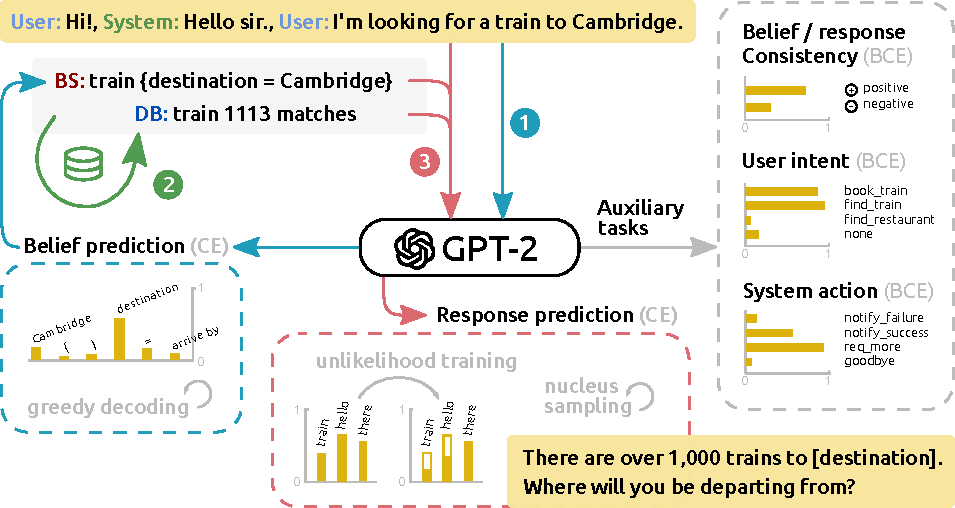
\includegraphics[width=0.8\textwidth]{schema_v3} % Reduce the figure size so that it is slightly narrower than the column. Don't use precise values for figure width.This setup will avoid overfull boxes.
\caption{The architecture of \augpt. The pipeline runs in two stages. First, a finetuned GPT-2 LM is used to predict a belief. Then the database results are obtained and everything is passed to the GPT-2 again to predict a final delexicalized response, along with possible auxiliary tasks (belief consistency, intent classification, system action classification). Unlikelihood loss is used for response prediction training.}
\label{fig:pipeline}
\end{figure*}

The task-oriented setting requires the dialogue system to respond adequately to the user's input and fulfill its goal. The goal could be, e.g., \ booking a train or requesting restaurant details. To achieve that, the system has to process the user's input, keep track of the belief state with respect to user preferences regarding individual in-domain attributes (slots) and generate a relevant response in natural language. The system also must be able to interact with an external database to incorporate the necessary information into the generated response (see Figure~\ref{fig:pipeline} for an example).

Due to its excellent language modeling and language generation capabilities, we have chosen the pre-trained GPT-2 LM as our system's backbone architecture. Similarly to \citet{budzianowski2019}, we use the LM to model both the belief state and the response.

\subsection{Model Representation}
\label{sec:model-repres}

The training instances for an LM-based task-oriented dialogue system can be considered as tuples $(c, b, d, r)$, where $r$ is the system's response, $c$ is the context (i.e., a concatenation of all previous utterances in the dialogue – both system's and user's), $b$ is the system's belief state which is also used for querying the database, and $d$ are the database results. 

In our case, the dialogue system handles multiple domains and the belief state is a set of pairs (\emph{domain name}, \emph{domain belief}), where the \emph{domain belief} is an assignment of values into slots, i.e., a set of pairs (\textit{slot name}, \textit{value}) (see \exampleref{ex:augpt_format}). Similarly, the database results $d$ are a set of pairs (\textit{domain name}, \textit{domain database results}), where the \textit{domain database results} are an ordered list of entities returned by the database. We further define the \emph{database result counts} $d_c$ denoting the number of results in $d$ for each domain.

Ideally, we would like our system to model the probability distribution over possible responses conditioned on the context $p(r|c)$. To simplify computation and model the interaction with an external database, this distribution can be factorized as follows:
\begin{equation}
\begin{split}
    p(r|c) &= \sum_{d} p(r|d,c) p(d|c) \\
           &= \sum_{d} \sum_{b} p(r|d,b,c) p(d|b) p(b|c) \\
           &= \sum_{b} p(r|\textit{Query}(b),b,c) p(b|c)\,,
\end{split}
\end{equation}
where $p(d|b)$ is a deterministic distribution over the database results, and \textit{Query} is a function returning database results.

By using this formulation and by modeling $p(r|d,b,c)$ and $p(b|c)$, our model would be able to process the context, query the database, and generate the response based on the database results. However, we would face a problem with data sparsity when estimating parameters of $p(r|d,b,c)$. The reason for the data sparsity is the relatively small size of datasets for task-oriented dialogues and the responses containing underrepresented, sometimes unique words, such as reference numbers, hotel names, etc. To maximally reuse the training samples, we choose to train our model on \emph{delexicalized responses} \cite{wen2015} denoted $\bar{r}$, where slot values are replaced with placeholders. During inference, the responses are lexicalized back deterministically using both the belief state and the database results. We assume perfect lexicalization, i.e., always being able to lexicalize the response $\bar{r}$ back based on $d$ and $b$.\footnote{We found in our experiments on the MultiWOZ data (see Section~\ref{sec:experiments}) that this assumption was almost always fulfilled.}


Both the database lookup and the lexicalization are deterministic, and the delexicalized response $\bar{r}$ does not depend on the database results $d$, but only on their counts $d_c$. Therefore, the distribution $p(r|d,b,c)$ is equal to the distribution $p(\bar{r}|d_c,b,c)$, and by maximizing its likelihood we are achieving the goal of maximizing the likelihood of $p(r|c)$.

We use the same language model $\hat{p}$ to model the belief state and to generate the delexicalized prediction. That is,
\begin{eqnarray}
    p(\bar{r}|d_c,b,c) & \approx & \hat{p}(\bar{r}|d_c,b,c,\theta) \\
    p(b|c) &  \approx&  \hat{p}(b|\emptyset,\emptyset,c,\theta)\,,
\end{eqnarray}
where we denote the model's parameters as $\theta$.

In the MultiWOZ dataset \cite[see Section~\ref{sec:experiments}]{budzianowski2018,eric2019}, responses are delexicalized by replacing concrete values with placeholder tokens of the form \textit{domain\_slot}. For better generalization across domains, we chose to use only \textit{slot} instead. We had noticed it was never the case that a response would involve more than one domain. Therefore, we decided to train our model to detect the \textit{active domain} and used the predicted active domain during the final lexicalization. The model predicts the active domain by outputting it as the first domain in the belief state. The other domains then follow in lexicographical order. The disadvantage of this approach is that we cannot determine the active domain if the belief state is empty. However, in such a case the lexicalization would fail anyway, so the system's performance is not affected by this decision.

\begin{example}
\begin{mdframed}[style=ExampleFrame]
%\begin{lstlisting}[columns=fullflexible,breaklines=true,breakindent=20pt,frame=tlrb,framextopmargin=0pt,framexbottommargin=0pt,framesep=0pt]
Belief state: train=\{ leave at=15:30, \\ 
\-\hspace{10pt}arrive by=17:15 \}, \\
\-\hspace{10pt}hotel = \{ price range = cheap \} \\
DB: train 23 matches, hotel no match
%\end{lstlisting}
\end{mdframed}
\caption{String format for \augpt's belief state and database result count\label{ex:augpt_format}.}
\end{example}

To generate the belief state and to input the database result counts to our model, we need a string representation. To fully exploit pre-training on natural language texts, we have chosen a compact representation containing as few special tokens as possible (see \exampleref{ex:augpt_format}).


\subsection{Model Training}
\label{sec:model-traning}
Although the parameters are shared for the belief state predictor and the delexicalized response predictor, the training objectives slightly differ. We use the cross-entropy loss for both predictions. For the response prediction, the unlikelihood loss \cite{welleck2019,li_dont_2020} is used as an additional objective. The unlikelihood loss gives a penalty for each repeated token, which helps the model avoid repetitions and makes frequent words less likely, increasing the answers' diversity.

To help the model learn a better internal representation from the data, we employ additional auxiliary tasks. Similarly to \citet{devlin2019} and \citet{peng2020}, we train a binary classifier to detect dialogue inconsistencies. In each training batch, we corrupt half of the samples by randomly applying one or more of the following changes with the same probability:
\begin{enumerate}
    \item We replace the belief state $b$ with another belief state, sampled uniformly randomly from the training data.
    \item We replace the delexicalized response $\bar{r}$ with a different randomly chosen one. If this change is applied in combination with the first one, the delexicalized response and the belief state are taken from the same random sample.
    \item A different valid value is uniformly sampled for each slot in the belief state. In this case, the domain names and domain order are unchanged (i.e., the active domain is the same).
\end{enumerate}
The first two changes are the same as those applied by \citet{peng2020}, whereas the third one is a new one which we find very useful in the context of multiple domains, where it is much more challenging to detect if the belief state was changed when the domain names are kept the same.
The consistency detection binary classifier is trained to recognize negative samples from the positive ones based on logits of the last response token. It is represented by an affine classifier trained using binary cross-entropy (BCE).

We also experiment with additional two classifiers predicting the user intent and the system action. These are implemented as two fully-connected layers attached to the feature representations of the last context token and the last database result token, respectively. 
However, based on our experimental results, we decided not to use these tasks in the final model.

We train the whole pipeline by optimizing the non-weighted sum of individual component losses, i.e., cross-entropy for the belief state and the response prediction, unlikelihood loss for the response, and BCE for the consistency detection are summed in our final system.

\subsection{Response Generation}
For each user input, the system transitions through several stages before the final response is generated. First, only the previous dialogue context is passed to the LM, which greedily generates the string representation of the belief state. The belief state is then parsed and passed to the database handler. The database handler then constructs a query and returns a set of results for each domain. We take the number of results for each domain and generate the string representation of database result counts (see \exampleref{ex:augpt_format}). All strings are concatenated and again passed to the language model. This time, we utilize the nucleus sampling \cite{holtzman2019} to generate the delexicalized response. We found nucleus sampling useful for generating the response since it increases diversity, but we prefer greedy decoding for the belief state with a fixed structure. Finally, the tokens in the delexicalized response are substituted by values from the database results and the belief state. The process is illustrated in Figure~\ref{fig:pipeline}.

\subsection{Data Augmentation}
Following its successful usage in other NLP tasks, \cite{konstas_neural_2017,elder_shape_2020}, we experiment with data augmentation using paraphrases, i.e., variants of training utterances with different surface forms.
In our setup, we generate multiple paraphrases for each training utterance and use them to augment the training data.
This way, we effectively increase the variability of the data.

Generating paraphrases is not a trivial process.
Various data-driven approaches were proposed, the majority of them corpora-based \cite{madnani2010generating}.
Recently, machine translation systems proved strong performance in generating paraphrases using the back-translation procedure \cite{sennrich2016,edunov2018,federmann2019multilingual}.
We take advantage of these findings and use a trained multilingual machine translation model \cite{machavcek2020elitr,edunov2018} to paraphrase our data.
We employ ten intermediate languages and thus obtain a set of different paraphrases for each input utterance.
When training, we choose the input user utterance uniformly at random from the set of all variants of the utterance including the original one.

\section{Experiments}
\label{sec:experiments}
\begin{table*}[htbp]
    \centering
    \begin{tabular}{l|ccc|ccc}
      \toprule
      & \multicolumn{3}{c|}{MultiWOZ 2.0} & \multicolumn{3}{c}{MultiWOZ 2.1} \\
      method & inform & success & BLEU & inform & success & BLEU \\
      \midrule
      Human & 91.0 & 82.7 & -- & 86.3 & 79.1 & -- \\
      \midrule
      \textbf{\Augpt} & 90.2 & 75.5 & 17.2 & 91.4 & 72.9 & 17.2 \\
      SOLOIST \cite{peng2020} & 85.5 & 72.9 & 16.5 & -- & -- & -- \\
      SimpleTOD \cite{hosseini2020} & 84.4 & 70.1 & 15.1 & 85.0 & 70.5 & 15.2 \\
      LABES-S2S \cite{zhang2020end2end} & -- & -- & -- & 78.1 & 67.1 & 18.3 \\
      DAMD \cite{zhang2019} & 76.3 & 60.4 & 16.6 & -- & -- & -- \\
      MD-Sequicity \cite{zhang2019} & 86.6 & 71.6 & 16.8 & -- & -- & -- \\
      LAVA \cite{lubis-etal-2020-lava} & 91.8 & 81.8 & 12.03 & -- & -- & -- \\
    %  UBAR \cite{yang2020ubar} & 95.4 & 80.7 & 17.0 & 95.7 & 81.8 & 16.5 \\
      \bottomrule
  \end{tabular}
  \caption{Comparison with previous works on the MultiWOZ dataset (see Section~\ref{sec:corpus-based} for a description of the metrics). \emph{MD-Sequicity} is a variant of \citet{lei2018}'s model, extended for a multi-domain setting.}
  \label{tab:multiwoz_sota_comparison}
\end{table*}
\begin{table*}[htbp]
    \centering
    \begin{tabular}{l|ccc|ccc|cc}
      \toprule
       &  & & & \multicolumn{3}{c|}{inform} & \multicolumn{2}{c}{turn} \\
      method & complete & success & book & P & R & F1 & succ & all \\
      \midrule
      \textbf{\Augpt} & 89.4 & 60.1 & 85.7 & 64.5 & 82.1 & 70.3 & 12.7 & 14.6 \\
      DAMD \cite{zhang2019} & 39.5 & 34.3 & 51.4 & 60.4 & 59.8 & 56.3 & 15.8 & 29.8\\
      Sequicity \cite{lei2018} & 23.1 & \phantom{0}9.8 & \phantom{0}4.1 & 33.0 & 32.7 & 29.9 & 12.2 & 32.6 \\
      \bottomrule
  \end{tabular}
  \caption{ConvLab evaluation comparison with other works (see Section~\ref{sec:convlab-eval} for a description of the metrics).}
  \label{tab:multiwoz_convlab_comparison}
\end{table*}


We consider a series of experiments to compare our model to current state-of-the-art methods, and include human evaluation and detailed error analysis.
We also carefully evaluate all proposed contributions through a series of ablation experiments.
%Moreover, we have obtained human evaluation results.

\subsection{Datasets}
We have used several datasets for training our system and for the final evaluation and comparison. 

We use \multiwozn, an enhanced version of \multiwoz \cite{budzianowski2018} that reduces the amount of noise in the data; we also use the 2.0 version in additional experiments so that we can compare to previous works.
The dataset contains 7 distinct domains (all related to tourist information, e.g., hotels, restaurants) and 10,438 dialogues, 7,032 of which are multi-domain.

%The \multiwozn contains dialogue state labels as well as annotation of dialogue acts and booking information.

We experiment with pre-training our model on additional datasets.
For the pre-training phase, we use \taskmaster \cite{byrne2019} and \schema \cite{rastogi2019}.
Both \taskmaster and \schema are multi-domain, task-oriented, large dialogue corpora consisting of 12,215 and 22,825 dialogues, respectively.
\taskmaster was obtained using the Wizard-of-Oz and self-dialogue methods, while the collection of \schema is somewhat artificial -- humans are only employed to paraphrase machine-generated utterances.
There are also other large-sized task-oriented datasets such as MetalWOZ \cite{lee2019multi}, however, they do not provide detailed annotation  to be able to exploit the data.

\subsection{Data Preprocessing}\label{sec:preprocessing}

Although the MultiWOZ 2.1 dataset was collected by humans, it contains a lot of inconsistencies. We hypothesize that when using only \textit{clean} samples which are consistent with the database, the benefit of using higher quality training data outweighs the decrease in the number of training samples. This claim is further supported by experiments (see the Ablation section). To filter the training data, we choose only those dialogues where the annotated dialogue goal corresponds with the turn-level annotated data. When using the \emph{clean} samples, we omit about 30\% of the training data.


To effectively combine all our datasets, we unified the domain-slot pairs in the belief states and the delexicalization.
%
However, the datasets use different naming conventions (e.g., \code{leaveAt} vs.\ \code{leave\_at}) and different domain and slot names even though the corresponding domain-slot pairs describe the same concepts (e.g., \code{restaurant-food} vs.\ \code{restaurant-type}). Therefore, we created a new unified ontology and manually designed a mapping between slot names. Notably, we decided to rename some slots so they use natural language tokens, as we base our model on the GPT-2 LM which is pre-trained on natural language texts (e.g. ``\code{leaveAt}''~$\rightarrow$~``\code{leave at}'').
Our final ontology that unifies all three datasets contains 22 domains and 135 slots. % distinct slots. 
%reduces the total number of domains from 76 to 22. 

We use our own implementation of delexicalization, which directly produces our belief state string representation (see Section~\ref{sec:model-repres} and \exampleref{ex:augpt_format}). % -- it removes the domain from the tokens and translates the tokens into natural language.


\subsection{Training Details}

We implement our model in the PyTorch framework \cite{pytorch}.
The model extends the \emph{small} variant of the GPT-2 model.
It consists of 12 transformer blocks with a model layer size equal to 768, having 124 million parameters in total.
For all auxiliary tasks, we use a dropout of 0.1 with label smoothing 0.1.
We use the AdamW optimizer \cite{loshchilov2017decoupled}.
For greater training effectiveness, we employ mixed-precision training \cite{micikevicius2017} through PyTorch AMP. 
The finetuning runs for 8 epochs on the \multiwozn data when all the training examples are used, and for the corresponding number of minibatches if a lower number of samples is used when using only \emph{clean} samples.
The training takes less than one day when using 4 GPUs.

\begin{table*}[t]
    \centering\small
    \begin{tabular}{lcccccc}
      \toprule
      & Average & Success & Success  & NLU &  Response & \\
      Method & Success & w/ DB & w/o DB & score & appropriateness & Turns \\
      \midrule
      Baseline & 69.6 & 56.8 & 82.4 & 4.34 & 4.18 & 18.5 \\
      Winner & \textbf{74.8} & \textbf{70.2} & 79.4 & \textbf{4.54 }& \textbf{4.47} & 18.5 \\
      Our submission & 72.3 & 62.0 & \textbf{82.6} & 4.53 & 4.41 & \textbf{17.1} \\
      \bottomrule
    \end{tabular}
    \caption{Human evaluation results obtained during the shared task using Amazon Mechanical Turk. Note that only 4 submissions outperformed the Baseline according to the average success metric.}
    \label{tab:human}
\end{table*}

\subsection{Corpus-based Evaluation}
\label{sec:corpus-based}

To compare with previous results on MultiWOZ, we evaluate the model performance with a set of corpus-based intrinsic metrics on both versions of the data.
In the case of MultiWOZ 2.0, we use the original delexicalization used also by other compared methods \cite{peng2020,hosseini2020,zhang2019}. For MultiWOZ 2.1, we use our own delexicalization.
We employ the original evaluation scheme by \citet{budzianowski2018}, which provides two metrics -- the \emph{inform rate} and the \emph{success rate}. The \emph{inform rate} is the percentage of dialogues in which the system provided an appropriate entity, whereas the \emph{success rate} is the percentage of dialogues in which the system outputted all the requested information. Additionally, we compute the BLEU score \cite{papineni2002} between the generated system utterances and the ground truth to get an approximation of the output fluency.
Note that both the \emph{inform rate} and the \emph{success rate} are unaffected by using a different delexicalization and these metrics can be directly compared to other methods. A different delexicalization could, however, render a slightly different BLEU, but based on preliminary results, we believe this change has almost no effect.


\subsection{ConvLab~2 Evaluation}
\label{sec:convlab-eval}

We use the ConvLab~2 platform \cite{zhu2020} for automatic evaluation.
The platform includes an agent-based evaluation component, therefore we obtain results gathered from interaction between our system and the simulated user agent.
We run the evaluation component 1,000 times, i.e.\ on 1,000 simulated conversations.
The agent mimics user behavior, interacts with the system under evaluation, and computes multiple metrics, among which the most relevant are \emph{complete}, \emph{success} and \emph{book} rates.
% https://github.com/thu-coai/ConvLab-2/blob/master/convlab2/policy/rule/multiwoz/policy_agenda_multiwoz.py
The \emph{complete rate} reflects the ratio of dialogues that are completed, i.e. all the user requests have been met.
% https://github.com/thu-coai/ConvLab-2/blob/master/convlab2/evaluator/multiwoz_eval.py
The \emph{success rate} computes the percentage of dialogues which are successful, meaning the system captures correct informed entities and provides a valid booking if requested.
Finally, the \emph{book rate} is the proportion of dialogues where the system was able to book the correct entity (hotel, restaurant, train) if it was asked to.
We also compute \emph{precision, recall} and \emph{F1 score} for the informed entities and the average number of turns in the dialogue.

\subsection{Human Evaluation and Error Analysis}

Thanks to our participation in a task-oriented dialogue shared task, the best one of our submissions was evaluated by human judges on the Amazon Mechanical Turk platform. The judges communicated with the agent in natural language and rated the system afterward with respect to the success/failure of the dialogue, language understanding score, and response appropriateness. Information provided by the system was additionally checked for consistency with the database, and the average of success rates given by the judges and by database grounding is used as the main metric.
%We refer to \citet{gunasekara2020overview} for more details.

In addition to the crowdsourced evaluation, we perform a detailed in-house error analysis of the model behavior based on human interactions with our final system. Expert annotators followed randomly chosen dialogue goals accompanying the MultiWOZ test set and recorded any incorrect system behavior.


\section{Results}
\label{sec:results}

In this section, we first describe and discuss the quantitative results for both corpus-based and crowdsourced human evaluation.
In the second part, we also perform a qualitative analysis of the model behavior.

\subsection{Comparison to State-of-the-Art on MultiWOZ}

Table \ref{tab:multiwoz_sota_comparison} shows a comparison between our methods and current state-of-the-art systems, which are described in the Related Work section.
Since \multiwozn has been released quite recently and some of the compared methods do not provide results with this version, we report results on both \multiwoz and MultiWOZ 2.1.
As we can see, \augpt outperforms all other approaches in terms of the \emph{inform} and \emph{success} metrics. However, DAMD and LABES-S2S produce higher BLEU scores.
This would indicate better fluency of these models, however, one would need human evaluation to confidently claim that.
One possible reason for this behavior would be our removal of some training samples (see Data Preprocessing), which may have decreased the BLEU score.
Importantly, thanks to the higher \emph{success} metric, we can say that our model is better at providing all the necessary information in the responses.

Table~\ref{tab:multiwoz_convlab_comparison} shows a comparison with two other models in the ConvLab evaluation scheme with a simulated user. The compared systems were chosen because they both implement fully trainable end-to-end methods. Our system outperforms both compared systems by a wide margin. Our model is able to perform well not just in a single-turn response generation scenario, but over the course of the whole dialogue. As the example of DAMD shows, this is not always guaranteed.

\begin{table*}[t]
    \centering\small
    \begin{tabular}{lc|ccccc}
      \toprule
      & Erroneous & BS & DB & Policy & Other \\
      & Dialogues  & Error & Error & Error & Error \\
      \midrule
      All dialogues & 50  & 30 & 4 & 21 & 6 \\
     % \% total & 100\% & 53.1\%  & 49.2\% & 7.9\% & 33.3\% & 9.5\% \\
     % \hdashline[1pt/2pt]
      Unsuccessful dialogues & 17 & 10 & 3 & 2 & 2 \\ 

      \bottomrule
    \end{tabular}
    \caption{Interactive  analysis performed by human evaluators using 130 prepared dialogue goals. 17 of these dialogues contained an error that caused the dialogue to fail. We show summary statistics regarding the number of respective error sources (BS = belief state, DB = database).
    Note that some of the dialogues contain more than one error.}
    \label{tab:interact_eval}
\end{table*}

% \begin{table*}[ht]
%     \centering\small
%     \begin{tabular}{lcccccccccc}
%       \toprule
%       & Hallucinated & Wrong & Missing & Ignored & Bad & False & Repeated & Failed&  \\
%       & Values       & Lex. & Info     & Input  & Dom. & Resp. & Output & Booking & Other \\
%       \midrule
%       frequency & 33.9\% & 9.6\% & 8.1\% & 8.1\% & 6.4\% & 6.4\% & 4.9\% & 4.9\% & 17.7\%
%       count & 21 & 6 & 5 & 5 & 4 & 4 & 3 & 3 & 10\\
%       \bottomrule
%     \end{tabular}
%     \caption{Distribution of the most common error types encountered during the human evaluation.}
%     \label{tab:detailed_eval}
% \end{table*}

\begin{table*}[t]
\centering\small
\begin{tabularx}{\textwidth}{lrcX}
\toprule
Type & Count & Source & Description \\
\midrule
Hallucinated values & 21 & BS/Policy & Used a slot value in the reply that is not grounded in the DB nor in the context \\
Wrong lexicalization & 6 & Policy & Repeats the same value in a list of choices during lexicalization  \\
Missing information & 5 & Policy & Makes booking while not all information is specified \\
Ignored input  & 5& BS & Keeps asking for information that was provided \\
Bad domain     & 4 & BS  & Fails to focus on the correct domain \\
False response & 4 & Policy & States a different value of a slot than the value stored in DB \\
Repeated output& 3 & Policy & Repeats the same slot twice on the output \\
Failed booking & 3 & DB/Policy & Booking was unsuccessful due to DB mismatch\\
Other          &10 & BS/DB/P/Oth & (Various rare errors that could not be categorized) \\
\bottomrule
\end{tabularx}
\caption{Distribution of the most common error types encountered during the human evaluation of 130 dialogues. Absolute counts of errors in the 50 erroneous dialogues are shown. The total error count is 61 as some dialogues contained multiple errors. The most likely source of the error (cf.~Table~\ref{tab:interact_eval}) and a short description are given for each type.}
\label{tab:detailed_eval}
\end{table*}

\subsection{Human Evaluation}

We show the human evaluation results in Table~\ref{tab:human}.
%The primary metric here was the \emph{Average success}.
Our model outperformed the baseline on the main average success metric (along with only half of other submissions).
We did not match the winning submission in terms of average success, but we achieved the best overall success rate based on human judgments (without checking consistency with the database).
This suggests that the biggest drawback of our model was the integration with database grounding.
This can be caused by our modified delexicalization, which makes it harder in some cases to match the database properly.
In addition, our model 
%However, our model performed well in the scenario when the database was not considered and 
needed the smallest number of turns overall to complete the evaluation dialogues.

We note that out of 5 submitted model variants in the competition (cf.~Table~\ref{tab:ablation_comparison}), only the model variant scoring best in the automatic evaluation was considered for human evaluation.
In our case, the chosen model variant did not include additional data pre-training, which could possibly improve performance in the human evaluation scenario.

%\begin{table*}[ht]
%    \centering\small
%    \begin{tabular}{lc|ccccc}
%      \toprule
%      & Total & No & BS & DB & Policy & Other \\
%      & Dialogues  & Error  & Error & Error & Error & Error \\
%      \midrule
%      count & 130 & 69  & 30 & 4 & 21 & 6 \\
     % \% total & 100\% & 53.1\%  & 49.2\% & 7.9\% & 33.3\% & 9.5\% \\
     % \hdashline[1pt/2pt]
%      no. successful & 113 & 69 & 20 & 1 & 19 & 4 \\ 
%      \% successful & 86.9\% & 100\% & 66.7\% & 25\% & 90.5\% & 66.7\% \\

 %     \bottomrule
 %   \end{tabular}
 %   \caption{Interactive  analysis performed by human evaluators using prepared dialogue goals. We show summary statistics regarding the number of respective error and compute a percentage of successful dialogues for each type of error.}
 %   \label{tab:interact_eval}
%\end{table*}

\subsection{Detailed Error Analysis}

\begin{example}[tpbh]
\small
\setlength{\tabcolsep}{2pt}
\begin{mdframed}[style=ExampleFrame]
\begin{tabularx}{\textwidth}{rX}
% Dialog 25
[...] \\
\bf user: & \it I want to make a booking at sitar tandoori \\
\bf belief: & restaurant \{name = sitar tandoori\} \\
& train \{arrive by = 18:00, day = sunday, departure = cambridge, destination = london liverpool street, people = 1\} \\
\bf system: & What day would you like the booking for? \\
\bf user: & \it the same day, 13:30 \\
\bf belief: & restaurant \{day = sunday, name = sitar tandoori, people = 1, time = 13:30\} \\
& train \{arrive by = 18:00, day = sunday, departure = cambridge, destination = london liverpool street, people = 1\} \\
\bf system: & Booking was successful. The table will be reserved for 15 minutes. Reference number is: 00000200. \\
\end{tabularx}
\end{mdframed}
\caption{A dialogue where the system did not ask for necessary information. The user previously booked a train trip for one person (cf.~the belief state in the first turn shown). When they went on to book a restaurant, the system took over the number of persons from the train ride and did not ask again.\label{ex:error1}}
\end{example}
\begin{example}[tpbh]
\small
\setlength{\tabcolsep}{2pt}
\begin{mdframed}[style=ExampleFrame]
\begin{tabularx}{\textwidth}{rX}
% dialogue 16
\bf user: & \it I'm looking for a theatre in Cambridge \\
belief: & attraction \{type = theatre\} \\
system: & There are 5 theatres in Cambridge. Is there an area of town you prefer? \\
\bf user: & \it no I don't care \\
belief: & attraction \{type = theatre\} \\
system: & I recommend Adc Theatre in the centre. Would you like more information? \\
\bf user: & \it no, I'm also looking for some place to stay \\
belief: & attraction \{type = theatre\} \\
\bf system: & I have 5 theatres in the centre. Do you have a price range? \\
\bf user: &  \it I'm looking for a place to stay \\
belief: & attraction \{type = theatre\} \\
\bf system: & There are 5 theatres in the centre. Do you have a preference for area? \\
\bf user: & \it I'm looking for a hotel \\
belief: & hotel \{type = hotel\} \\ 
& attraction \{type = theatre\} \\
\bf system: & \it There are 9 hotels in the north. Do you have a price range?\\
\end{tabularx}
\end{mdframed}
\caption{Dialogue sample with a bad domain focus and a hallucination. First, the system ignores that the user switched from searching for a theater to searching for a hotel. After accepting the new domain, the system replies with hotels “in the north” even though the user did not specify.\label{ex:error2}}
\end{example}

\begin{example}[t]
\small
\setlength{\tabcolsep}{2pt}
\begin{mdframed}[style=ExampleFrame]
\begin{tabularx}{\textwidth}{rX}
\bf user : & I am looking for a cheap \textit{chinse} restaurant. \\
\bf belief: & restaurant \{food = chinese, price range = cheap\} \\
\bf system: & I have 4 cheap chinese restaurants. What area of town would you like to dine in?\\
\bf user: & downtown   \\ 
\bf belief: & restaurant \{area = centre, food = chinese, price range = cheap\} \\
\bf system: & I have 3 cheap chinese restaurants in the centre. Would you like to book at Charlie Chan?\\
 & ... \\

\end{tabularx}
\end{mdframed}
\caption{A snippet from challenging yet successful dialogue. The system deals with input noise (chinse) as well as with paraphrases (downtown). \label{ex:success}}
\end{example}

\begin{table*}[tp]
    \centering\small
    \begin{tabular}{l|ccc|ccc|ccc|cc}
      \toprule
        & \multicolumn{3}{c|}{MultiWOZ 2.1} & \multicolumn{8}{c}{ConvLab 2}  \\
       & \multicolumn{3}{c|}{} & \multicolumn{3}{c}{} & \multicolumn{3}{c}{inform} & \\
      method \text& inf & suc & BLEU & \hspace{-1mm}comp\hspace{-1mm} & \hspace{-1mm}suc\hspace{-1mm} & book & P & R & F1 & turns \\
      \midrule
      \textbf{\augpt} & $\mathbf{91.4} \pm .1$ & $72.9 \pm .1$ & $17.2 \pm .02$ & \textbf{89.4} & \textbf{60.1} & 85.7 & 64.5 & \textbf{82.1} & 70.3 & 14.6 \\
    \midrule
    w/o. unlikelihood & $91.3 \pm .1$ & $71.8 \pm .1$ & $16.9 \pm .02 $ & 89.2 & 59.3 & \textbf{90.8} & 63.9 & 81.6 & 69.5 & 14.6 \\
    w/o. clean & $\mathbf{91.5} \pm .1$ & $70.8 \pm .1$ & $15.8 \pm .02$ & 85.0 & 57.7 & 85.6 & 65.6  & 79.1 & 69.6 & 14.5 \\
    w/o. unlikelihood, clean & $90.9 \pm .1$ & $\mathbf{74.2} \pm .1$ & $\mathbf{17.5} \pm .02$ & 85.9 & 58.4 & 81.3 & 62.2 & 79.8 & 67.5 & \textbf{14.1} \\
    w. all auxiliary & $91.4 \pm .1$ & $72.5 \pm .1$ & $16.8 \pm .02$ & 88.7 & 59.2 & 86.0 & 64.6 & 81.1 & 69.9 & 14.4 \\
    \midrule
    w/o. pre-training & $90.8 \pm .1$ & $68.9 \pm .1$ & $15.1 \pm .02$ & 88.1 & 59.8 & 83.7 & \textbf{68.1} & 80.9 & 72.1 & 15.6 \\
    % base & 91.0 & 75.5 & 16.73 & 84.8 & 58.2 & 84.7 & 62.2 & 79.3 & 67.3 & 13.0 & 15.3\\
    % clean & 90.3 & 68.7 & 16.50 & 87.6 & 58.8 & 85.3 & 63.7 & 79.9 & 68.7 & 13.2 & 15.3 \\
    % unlike & 90.7 & 74.6 & 15.52 & 86.3 & 59.1 & 81.4 & 67.3 & 80.1 & 71.1 & 13.0 & 14.8 \\
    % rainbow & 91.2 & 72.5 & 15.52 & 86.4 & 59.9 & 88.1 & 66.9 & 80.5 & 70.9 & 13.3 & 15.3 \\
    % \midrule
    w/o. back-translations & $89.4 \pm .1$ & $69.2 \pm .1$ & $15.2 \pm .02$ & 88.9 & 58.2 & 87.4 & 68.0 & 81.6 & \textbf{72.2} & 14.9 \\
    % clean-pre-noback & 89.7 & 70.3 & 16.5 & 85.8 & 57.4 & 79.8 & 65.5 & 80.1 & 70.1 & 13.0 & 15.0 \\
    % base-pre-noback & 90.2 & 68.4 & 16.6 & 82.0 & 56.9 & 70.6 & 63.7 & 79.0 & 68.4 & 13.2 & 14.7 \\
    % rainbow-pre-noback & 88.8 & 68.1 & 16.8 & 86.9 & 58.1 & 84.2 & 64.6 & 80.8 & 69.6 & 12.8 & 14.8 \\
    w. old consistency & $91.0 \pm .1$ & $72.5 \pm .1$ & $17.0 \pm .02$ & 85.5 & 57.8 & 86.0 & 65.2 & 80.0 & 69.8 & 14.6  \\
    w/o. consistency & $90.5 \pm .1$ & $69.5 \pm .1$ & $16.3 \pm .02$ &  86.4 & 57.1 & 84.1 & 66.3 & 81.2 & 70.9 & 14.6 \\
    \bottomrule
  \end{tabular}
  \caption{Ablation study (inf = inform, suc = success, book = book rate; see Section~\ref{sec:corpus-based} for a description of metrics). The model version with the best ConvLab~2 success rate is chosen as our best model. Variants are denoted with their respective modifications compared to the default: ``w/o.\ unlikelihood'' = unlikelihood loss was not used for training; ``w/o.\ clean'' uses all training samples as opposed to using only the ones consistent with the database; ``w/o.\ pre-training'' = the additional Taskmaster-1 and Schema-Guided datasets were not used for training; ``all auxiliary'' = using two additional auxiliary tasks (see the Method section for details); ``w/o.\ consistency'' = dialogue consistency task is not used; ``old consistency'' refers to the consistency task as defined by \citet{peng2020} (see the Section~\ref{sec:model-traning} for details).}
  \label{tab:ablation_comparison}
\end{table*}


Our expert annotators evaluated 130 dialogues in total, 50 of which contained at least one error.
However, in most cases, the system was able to recover from the errors, resulting in an overall success rate of 86.9\% (i.e., 17 unsuccessful dialogues).

The purpose of this analysis was to find out what kind of errors occur during real interaction.
The annotators were familiar with the model architecture and were instructed to categorize the errors according to the cause of the problem.
Specifically, they identified which component caused the respective error based on the internal system state.
In addition, the annotators categorized the errors into more specific types. %, such as like \emph{hallucinated values}, \emph{wrong lexicalization} or \emph{missing information}. 

The overall results are given in Table~\ref{tab:interact_eval}.
We observe that the most common reason for a failed dialogue is an error related to the belief state.
Also, although policy errors happen relatively often, they rarely cause the whole dialogue to fail.
We observe that we have a slightly higher number of successful dialogues compared to the 82.6\% success rate (without checking database consistency) found in human evaluation (cf.\ Table~\ref{tab:human}).
The most likely cause of this behavior is that our expert annotators were more motivated to recover from erroneous system behavior and finish the dialogue.
%There are two likely causes of this: (1) The expert annotators used dialogue goals accompanying the MultiWOZ data, i.e. the same type of goals that were used to collect the training set. Using known types of situations makes it easier for the model

Fine-grained error types identified by annotators are given in Table~\ref{tab:detailed_eval}. We now provide examples for some of the frequent types which deserve more detail.
By far the most common error was \emph{hallucinated values} -- lack of grounding for some of the information provided (see the end of \exampleref{ex:error1}). One of the causes of this error, as in the case of this example, were hallucinations coming from the decoder. This probably stems from an imperfect delexicalization of some of the training samples.
Another error type is \emph{missing information}, i.e., not asking for information that is required (\exampleref{ex:error2}). In this case, the system uses information from a different domain without the user explicitly confirming this.
% (number of people was taken from trains to restaurants in the example).
A most probable cause of this is that most instances of the training data carry over the information.
A third common error type is \emph{bad domain} (see the beginning of \exampleref{ex:error1}). Here, the system does not react to the user's request for a different search (hotels instead of attractions in the example). This might be caused by a less frequent wording of the request in the given context, and usually gets resolved by rephrasing the request.

Apart from the errors, many examples of non-trivial positive behavior were found during the analysis. As illustrated in Example~\ref{ex:success},
the model is able to deal with paraphrases and is robust to a certain amount of noise in the data. Specifically, it handles typos, various time formats, etc.
Interaction between domains is also successful in most cases -- the system is able to resolve references to another domain's belief state (e.g., make a booking for the same group of people as done before in a different venue).
%The system can also resolve references to another domain's belief state. For instance, the system understands the request to make the reservation for the same group of people as it has done before in a different venue.


\section{Ablation Study}
We tested many variants of our method with different combinations of our proposed system's components to evaluate their contributions. The results are presented in Table \ref{tab:ablation_comparison}.
Namely, we are interested in the following components:
\textbf{(1)} the unlikelihood loss, \textbf{(2)} the auxiliary tasks, \textbf{(3)} the data augmentation, \textbf{(4)} the modified consistency task and \textbf{(5)} unclean data filtering.

We can see that all proposed contributions which are a part of our final system have a positive effect on the system performance with respect to the primary metrics.
We can see that removing either the pre-training or the back-translations decreases the BLEU score and, more importantly, the success rates. Furthermore, we notice the positive effect of using our improved consistency detection task over the one used in SOLOIST \cite{peng2020}, which in turn scores better than no consistency detection. 

Removing either the unlikelihood loss or training on all data as opposed to only “clean” samples clearly reduces performance.
However, we did not notice any increase in performance when the user intent prediction and system action prediction auxiliary tasks were used (cf.\ Section~\ref{sec:model-traning}).
The reason for this behavior could be that the model learns to represent the actions well enough implicitly, without the need for these additional objectives.
However, these tasks are not a part of our final model.

%One interesting aspect of the results is that the book rate did not correspond well with the success rate. This inconsistency might be caused by the ConvLab 2 evaluation itself, where the database used by the ConvLab 2 user agent expected an exact wording of the response returned by our system.

%TODO: add caption
\begin{table*}
    \centering\small
    \begin{tabular}{ll|cc|ccc|cc}
        & & \multicolumn{2}{c|}{oracle} & \multicolumn{3}{c|}{DST} & \multicolumn{2}{c}{NLG} \\
        fine-tuned on & evaluated on & bs & db & joint acc. & slot acc. & F1 & BLEU & ROUGE-L \\
        \hline
        \multirow{3}{*}{MW 2.0} & \multirow{3}{*}{MW 2.0} & \xmark & \xmark & \multirow{3}{*}{54.1} & \multirow{3}{*}{97.2} & \multirow{3}{*}{90.0} & 22.1 & 42.4 \\
        && \xmark & \cmark &  & & & 22.3 & 42.6 \\
        && \cmark & \cmark &  & & & 22.3 & 42.6 \\
        \hline
        \multirow{3}{*}{MW 2.1} & \multirow{3}{*}{MW 2.1} & \xmark & \xmark & \multirow{3}{*}{56.5} & \multirow{3}{*}{97.2} & \multirow{3}{*}{90.6} & 23.2 & 42.2 \\
        && \xmark & \cmark &  & & & 22.4 & 42.4 \\
        && \cmark & \cmark &  & & & 23.4 & 42.4 \\
        \hline
        \multirow{2}{*}{TM + SG} & \multirow{2}{*}{TM} & \xmark & \cmark & \multirow{2}{*}{46.1} & \multirow{2}{*}{98.1} & \multirow{2}{*}{38.5} & 11.4 & 31.0 \\
        && \cmark & \cmark &  & & & 11.3 & 31.0 \\
        \hline
        \multirow{2}{*}{TM + SG} & \multirow{2}{*}{SG} & \xmark & \cmark & \multirow{2}{*}{.} & \multirow{2}{*}{...} & \multirow{2}{*}{...} & .. & .. \\
        && \cmark & \cmark &  & & & .. & .. \\
        \hline
    \end{tabular}
    \caption{Caption}
    \label{tab:my_label}
\end{table*}

\section{Conclusions \& Future Work}
We present a dialogue modeling pipeline based on the pre-trained GPT-2 language model.
\Augpt uses modified training objectives and employs data augmentation to increase the diversity of generated utterances.
Our experiments show that the proposed approach performs better than state-of-the-art baselines in a multi-domain scenario on the MultiWOZ dataset.
We also run a series of ablation experiments to assess the individual contributions of the modifications.
According to our detailed ablation study, 
training data augmentation using back-translation via multiple languages and a modified auxiliary training objective for dialogue consistency detection are the features that contribute most to our system's performance.
Additionally, we perform a qualitative analysis of the outputs to give a better insight into our model behavior.
%We participated in the DSTC9 shared task for multi-domain task-oriented end-to-end dialogue modeling.
%Our submission placed third in the final evaluation while obtaining the best results in the \emph{success} metric without database grounding and achieving the shortest dialogues on average.

% In the future work, we'll focus on exploiting the additional data sources for pre-training.

In the future, we plan to construct a latent representation of the belief state and optimize it jointly with the language model. We will replace the deterministic lexicalization with a trainable alternative, and possibly even integrate the database module into the model. To improve the transfer to new domains, we will learn a domain embedding and optimize it jointly with the model, unifying all datasets.


% \section*{Acknowledgements}

% Entries for the entire Anthology, followed by custom entries
\bibliography{bibliography}
\bibliographystyle{acl_natbib}

% \appendix
% \section{Example Appendix}
% \label{sec:appendix}
% This is an appendix.

\end{document}
